% -*- root: diplomarbeit.tex -*-
\section{Anhang}
\subsection*{OpenCV}
Die \textit{Open Source Computer Vision Library} OpenCV ist einen Bibliothek mit einer Sammlung von Klassen und Algorithmen in den Bereichen des machinellen Sehens, der Bildverarbeitung und des maschinellen Lernens implementiert und zur (meist) freien Verfügung stellt. Wurde anfangs nur die Sprache C unterstützt, gibt es heute ein Reihe von Implementierungen in C++, Python, Java und auch MATLAB. Außerdem werden sowohl die gängigen Betriebssysteme Windows, Linux und Mac OS, als auch das mobile OS Android unterstützt.

Zur Zeit befinden sich spezielle Module in der Entwicklung (basierend zum Beispiel auf CUDA), die es erlauben, Algorithmen expliziet auf der GPU (\textit{Graphic Processor Unit}), also auf dem Grafikprozessor, auszuführen. Die Auslagerung auf die für die Verarbeitung von Bilddaten optimierte Hardware hat vor allem Ge- schwindigkeitsvorteile (siehe Abbildung \ref{GPU_Performance}).

\begin{figure}
\centering{}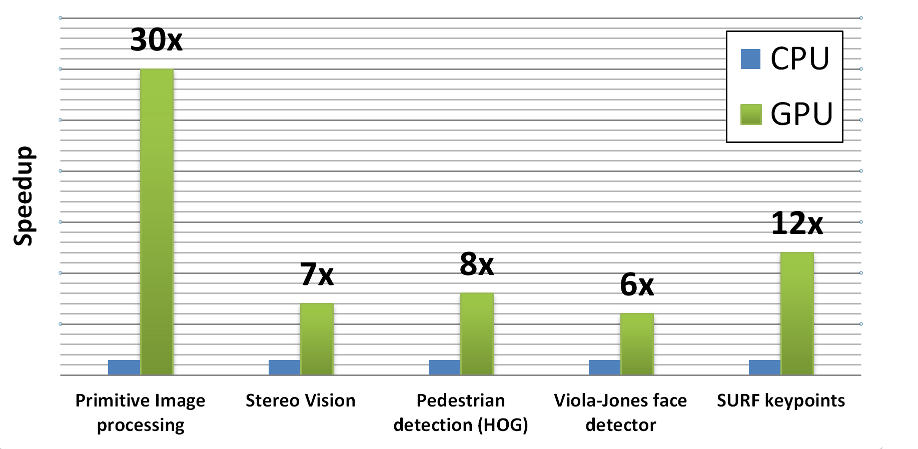
\includegraphics[scale=0.5]{../pictures/GPU_Performance.png}\caption{Tesla C2050 versus Core i5-760 2.8Ghz, SSE, TBB \cite{OCW}}
\label{GPU_Performance}
\end{figure}

\subsection*{OpenTLD}
Im Laufe der Bearbeitung des Themas wurde eine C++-Implementierung von TLD veröffentlicht. OpenTLD adaptiert die originale Matlab-Version, erweitert allerdings die Detector-Kaskade um einen weiteren Filter, den Foreground-Filter. Dieser dient in erster Linie zur Reduzierung der möglichen BoundingBoxes durch Subtraktion des Hintergrundes.

Mit Hilfe eines Forground-Filters kann ein sich bewegendes Objekt mittels Background-Substraction aus einer Videosequenz separiert werden{[}QUELLE{]}. Dieses Verfahren wird vor allem bei statischen Kameras verwendet, die fest montiert. In einer sehr dynamischen Anwendung, wie das Finden und Verfolgen von sich bewegenden Objekten mittels auf einem Flugroboter montierten Kamera unter Nichtlaborbedingungen, hat eine solche Komponente somit keine Relevanz auf die Robustheit des Algortihmus. Außerdem ist dieser Filter nicht Teil der originalen Veröffentlichung von Z. Kalal. Aus diesen Gründen wurde auf eine Implementierung verzichtet. Teile von OpenTLD wurden zu Analysezwecke und standen zur Vervollständigung der eigenen Implementierung Pate.

\subsection*{Algorithmen}
An dieser Stelle gibt es eine Übersicht der restlichen verwendeten Algorithmen.

\paragraph{Varianz-Classifier}
Der Varianz-Classifier berechnet in den Zeilen 1 und 2 das integrale beziehnugsweise das quadratische integrale Bild. Im Anschluss werde die Werte aus den acht Ecken der beiden Rechtecke ermittelt und der Mittelwert $mean$ und $mean^2$ berechnet. Die Varianz ergibt sich aus der Differenz $var = mean^2 - (mean\times mean)$ und wird im Detector mit dem Varianz-Threshold $\Theta$ verglichen. Gilt $var < \Theta$, wird $I$ verworfen

\begin{algorithm}[H]
	\vspace{0.2cm}
	\KwData{$I,x,y,w,h$}
	\KwResult{$var$}
	$I_{int} = calcIntegral(I)$\;
	$I^2_{int} = calcSqrtIntegral(I)$\;
	$br=I_{int}.at(x + w, y + h)$\;
	$bl=I_{int}.at(x, y + h)$\;
	$tr=I_{int}.at(x + w, y)$\;
	$ts=I_{int}.at(x, y)$\;
	$brs=I^2_{int}.at(x + w, y + h)$\;
	$bls=I^2_{int}.at(x, y + h)$\;
	$trs=I^2_{int}.at(x + w, y)$\;
	$tss=I^2_{int}.at(x, y)$\;
	$mean = (br + tl - tr - bl)/(w\times h)$\;
	$mean^2 = (brs + tls - trs - bls)/(w\times h)$\;
	$var = mean^2 - (mean\times mean)$\;
	\caption{Varianz-Classifier}
	\label{alg:varianz}
	\vspace{0.2cm}
\end{algorithm}

\paragraph{Ensemble-Classifier}
Hier die Erklärung des Algorithmus.

\begin{algorithm}[H]
	\vspace{0.2cm}
	\KwData{Input}
	\KwResult{Output}
	TODO
	\caption{Ensemble-Classifier: Train Classifier}
	\label{alg:ensemble_train}
	\vspace{0.2cm}
\end{algorithm}

\begin{algorithm}[H]
	\vspace{0.2cm}
	\KwData{Input}
	\KwResult{Output}
	TODO
	\caption{Ensemble-Classifier: Classify}
	\label{alg:ensemble_calc}
	\vspace{0.2cm}
\end{algorithm}

\paragraph{NearestNeighbour-Classifier}
Hier die Erklärung des Algorithmus.

\begin{algorithm}[H]
	\vspace{0.2cm}
	\KwData{Input}
	\KwResult{Output}
	TODO
	\caption{NearestNeigbour-Classifier: Train}
	\label{alg:nearest_neighbour_train}
	\vspace{0.2cm}
\end{algorithm}

\begin{algorithm}[H]
	\vspace{0.2cm}
	\KwData{Input}
	\KwResult{Output}
	TODO
	\caption{NearestNeigbour-Classifier: Classify}
	\label{alg:nearest_neighbour_calc}
	\vspace{0.2cm}
\end{algorithm}

\paragraph{Clustering}
Hier die Erklärung des Algorithmus.

\begin{algorithm}[H]
	\vspace{0.2cm}
	\KwData{Input}
	\KwResult{Output}
	TODO
	\caption{Clustering}
	\label{alg:cluster}
	\vspace{0.2cm}
\end{algorithm}